\documentclass[a4paper,12pt]{article}
\usepackage[T1]{fontenc}
\usepackage[utf8]{inputenc}
\usepackage{url}
\usepackage{fancyhdr}
\usepackage{lastpage}
\usepackage{hyperref}
\usepackage{graphicx}

\setlength\parindent{0pt}

\pagestyle{fancy}
\fancyhf{}
\lhead{Codeforces notes}
\cfoot{\thepage/\pageref{LastPage}}

\title{Codeforces notes}
\author{Mario Ynocente Castro (MarioYC)}
\date{}

\begin{document}

\maketitle
\thispagestyle{empty}

\newpage
\tableofcontents

\newpage
\section{\href{http://codeforces.com/contest/687}{Codeforces Round 360 (Div 1)}}

\subsection{The Values You Can Make}

We can use a DP with state (position, sum1, sum2) where we want sum1 to be $k$ at the end, and the different valid values of sum2 will be the answer.
\\ \\
\textbf{Implementation:} \href{http://codeforces.com/contest/687/submission/19365759}{C++ code}
\\ \\
\textbf{Note:} Should start by trying DP first before looking for a more complicated approach and check the amount of memory of the solution.

\subsection{Dividing Kingdom II}

In any interval sort the edges in decreasing order by their weight, then the important edges are the ones that join two different components and the first edge that joins vertices that are in the same component and apart from each other by an even number of edges, so the number of important edges is at most n.
\\ \\
We can build a segment tree that keeps the important edges for an interval, and then for each query we will do at most $\log n$ steps that consist of merging these sets of important edges.
\\ \\
\textbf{Implementation:} \href{http://codeforces.com/contest/687/submission/19196725}{C++ code}
\\ \\
\textbf{Notes:}
\begin{itemize}
\item
The same approach would work for similar problems like MST and number of connected components.
\item
The intervals that are going to be merged could intersect and it would still be correct, so we could use a sparse table and then only one merge per query would be necessary, but the complexity of the preprocessing will increase, since we no longer have the guarantee that each edge will be added at most $O(\log m)$ times.
\end{itemize}

\section{\href{http://codeforces.com/contest/690}{Helvetic Coding Contest 2016}}

\subsection{Brain Network (hard)}

Let $u$ and $v$ be the extreme vertices of the diameter and $w$ a new vertex we'll add,
we can prove that the new value of the diameter will be between $d(u,v), d(u,w)$ and $d(w,v)$.
\\ \\
If the length of the diameter increases then one of the new extreme vertices should be $w$,
and if the other extreme is a vertex $x$ which isn't $u$ nor $v$, then there
are two cases:

\begin{figure}[!ht]
\centering
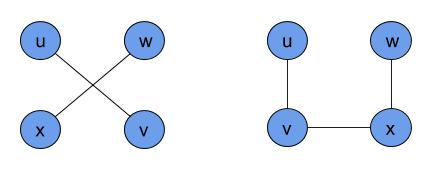
\includegraphics[scale=0.6]{img/helvetic-c.jpg}
\caption{Possible cases}
\end{figure}

In both cases we get contradictions.
\\ \\
\textbf{Implementation:} \href{http://codeforces.com/contest/690/submission/19389500}{C++ code}

\subsection{The Wall (hard)}

We can get the recurrence:

\begin{center}
$\forall i > 0, f(i) = \sum_{w = 0}^W (f(i - (w + 1)) \cdot H^w)$

$f(0) = f(-1) = 1$
\end{center}

which we can use to solve the problem using matrix exponentiation.
\\ \\
\textbf{Implementation:} \href{http://codeforces.com/contest/690/submission/19405468}{C++ code}
\\ \\
\textbf{Note:} Started with a DP state (pos, behind, have) to accumulate the length of all segments
in have, but fixing one segment at the time gave the simpler recurrence.

\section{\href{http://codeforces.com/contest/691}{Educational Codeforces Round 14}}

\subsection{Couple Cover}

If all $a_i$ are different and $P = 3 \cdot 10^6$ then the number of pairs $(i,j)$ for which $a_i a_j \leq P$ is $O(P\log P)$ and if these values are sorted then we can go through these pairs in $O(n + P\log P)$. For the general case, we will first need to compress these values.
\\ \\
While going through the values we can increase a counter for each different value of the product, then we can accumulate these counters.
\\ \\
\textbf{Implementation:} \href{http://codeforces.com/contest/691/submission/19352079}{C++ code}

\end{document}
